En este capítulo se presentan los resultados obtenidos a partir de la evaluación de la salida de la herramienta ClickUp, siguiendo la metodología descripta en el capítulo \ref{cap:evaluacion}.

\section{Salida de la herramienta ClickUp}
La salida de la herramienta sigue el formato indicado en el prompt \ref{fig:prompt_simple} y consta de historias de usuario, donde cada una incluye criterios de aceptación, referencia al documento e indicación de si es una épica, además de una sección final titulada Inconsistencies, Ambiguities, or Contradictions (Inconsistencias, ambigüedades o contradicciones). 

Las historias generadas se presentan en la tabla \ref{tab:historias_clickup}, junto a sus criterios de aceptación en la tabla \ref{tab:criterios_clickup}, las referencias al documento de requisitos en la tabla \ref{tab:referencias_clickup} e indicación de si es una épica en la tabla \ref{tab:epicas_clickup}.

Las inconsistencias, ambigüedades o contradicciones detectadas en el documento se presentan en la tabla \ref{tab:inconsistencias_clickup}.

\begin{longtable}{|c|p{12cm}|}
\caption{Historias Generadas por ClickUp} \label{tab:historias_clickup} \\
\hline
\textbf{Referencia} & \textbf{Historia de usuario} \\
\hline
\endfirsthead


\caption{Historias Generadas por ClickUp - Continuación} \\
\hline
\textbf{Referencia} & \textbf{Historia de usuario} \\
\hline
\endhead

\hline
\endfoot

\hline
\endlastfoot

HU1 & As an administrative staff member, I want to register patients with personal data and medical background, so that the hospital can maintain accurate and complete patient records. \\
\hline
HU2 & As an administrative staff member, I want to modify the personal and contact details of a registered patient, so that patient information remains up to date. \\
\hline
HU3 & As an administrative staff member, I want to search for patients by name, identity document, or identifier number, so that I can quickly locate patient records. \\
\hline
HU4 & As an authorized user, I want to visualize a patient's complete information, so that I can review all relevant details for care or administration. \\
\hline
HU5 & As an administrative staff member, I want to create medical appointments by associating the patient, specialty, and professional, so that appointments are scheduled accurately. \\
\hline
HU6 & As an administrative staff member, I want to visualize the availability of registered doctors, so that I can schedule appointments efficiently. \\
\hline
HU7 & As an administrative staff member, I want to modify or cancel existing appointments, so that changes can be managed as needed. \\
\hline
HU8 & As a patient, I want to receive notifications when my appointment is modified or canceled, so that I am always informed about my schedule. \\
\hline
HU9 & As an administrative staff member, I want to manage the status of appointments throughout their lifecycle, so that the hospital can track appointment outcomes. \\
\hline
HU10 & As a doctor, I want to register diagnoses, treatments, and patient’s clinical progress in the electronic clinical record, so that patient care is well documented. \\
\hline
HU11 & As a patient, I want to consult my electronic clinical record, so that I can stay informed about my health history. \\
\hline
HU12 & As an administrator, I want to register medical professionals with their personal and contact details and associate specialties, so that the hospital can manage staff information. \\
\hline
HU13 & As an administrator, I want to define and modify attention hours and activate or deactivate professionals for scheduling, so that doctor availability is accurately reflected. \\
\hline
HU14 & As an administrator, I want to manage roles and access permissions to system functionalities, so that users only access features relevant to their role. \\
\hline
HU15 & As an administrative staff member, I want to generate electronic invoices for medical consultations and medication delivery, so that billing is accurate and efficient. \\
\hline
HU16 & As a patient, I want to receive automatic notifications with attached digital invoices when an invoice is generated, so that I am promptly informed about charges. \\
\hline
HU17 & As a pharmacist, I want to register medications and supplies with identification, stock, and expiration date, so that inventory is accurately tracked. \\
\hline
HU18 & As a pharmacist, I want to automatically update stock when registering medication deliveries, so that inventory levels remain current. \\
\hline
HU19 & As a pharmacist, I want to be notified when stock is low or items are about to expire, so that I can take timely action. \\
\hline
HU20 & As a pharmacist, I want to consult inventory sorted by available quantity or expiration date, so that I can manage stock efficiently. \\
\hline
HU21 & As an analyst, I want to generate reports on consultations by specialty, appointment status, financial income, and medication and supplies consumption, with date range filters, so that I can analyze hospital performance. \\
\hline
HU22 & As a system administrator, I want to ensure date validations prevent invalid ranges, so that data integrity is maintained. \\
\hline
HU23 & As a system administrator, I want to ensure notifications are sent within a reasonable time after triggering events, so that users are promptly informed. \\
\end{longtable}

\begin{longtable}{|c|c|p{9cm}|}
\caption{Criterios de aceptación Generados por ClickUp} 
\label{tab:criterios_clickup} \\
\hline
\textbf{Referencia CA} & \textbf{Ref. HU} & \textbf{Criterio de aceptación} \\
\hline
\endfirsthead

\caption{Criterios de aceptación Generados por ClickUp - Continuación} \\
\hline
\textbf{Referencia CA} & \textbf{Ref. HU} & \textbf{Criterio de aceptación} \\
\hline
\endhead

\hline
\endfoot

\hline
\endlastfoot

AC1.1 & HU1 & The system allows entry of personal and medical background data \\
\hline
AC1.2 & HU1 & Each patient receives a unique identifier \\
\hline
AC1.3 & HU1 & Duplicate identity documents or identifiers are not allowed \\
\hline

AC2.1 & HU2 & The system allows editing of existing patient records \\
\hline

AC3.1 & HU3 & The system supports search by name, document, or identifier \\
\hline

AC4.1 & HU4 & The system displays all patient data in a single view \\
\hline

AC5.1 & HU5 & The system allows selection of patient, specialty, and doctor \\
\hline
AC5.2 & HU5 & Overlapping appointments are prevented \\
\hline

AC6.1 & HU6 & The system displays doctors’ schedules and availability \\
\hline

AC7.1 & HU7 & The system allows editing and canceling of appointments \\
\hline
AC7.2 & HU7 & Patients are notified of changes \\
\hline

AC8.1 & HU8 & Notifications are sent promptly after changes \\
\hline

AC9.1 & HU9 & Appointment statuses include Confirmed, Canceled, Attended, and Not attended \\
\hline

AC10.1 & HU10 & The system allows entry and editing of clinical records \\
\hline
AC10.2 & HU10 & Each entry is timestamped \\
\hline

AC11.1 & HU11 & Patients can view but not edit their records \\
\hline
AC11.2 & HU11 & Access is restricted to authorized users \\
\hline

AC12.1 & HU12 & The system allows entry and editing of staff data and specialties \\
\hline

AC13.1 & HU13 & The system supports setting and updating working hours \\
\hline
AC13.2 & HU13 & Professionals can be activated or deactivated for scheduling \\
\hline

AC14.1 & HU14 & The system enforces role-based access control \\
\hline
AC14.2 & HU14 & Permissions are validated before actions are executed \\
\hline

AC15.1 & HU15 & The system generates invoices with unique identifiers \\
\hline
AC15.2 & HU15 & Invoices are associated with patients and services \\
\hline

AC16.1 & HU16 & Notifications are sent with invoice attachments \\
\hline

AC17.1 & HU17 & The system allows entry of medication and supply data \\
\hline

AC18.1 & HU18 & Stock is updated in real time upon delivery \\
\hline

AC19.1 & HU19 & The system detects minimum stock and upcoming expirations and sends notifications \\
\hline

AC20.1 & HU20 & Inventory can be sorted by quantity or expiration \\
\hline

AC21.1 & HU21 & Reports include all specified metrics \\
\hline
AC21.2 & HU21 & Reports can be filtered by date range \\
\hline

AC22.1 & HU22 & The system does not allow invalid date ranges \\
\hline

AC23.1 & HU23 & Notifications are sent shortly after relevant events \\

\end{longtable}

\begin{longtable}{|c|c|p{9cm}|}
\caption{Referencias Generadas por ClickUp} 
\label{tab:referencias_clickup} \\
\hline
\textbf{Referencia R} & \textbf{Ref. HU} & \textbf{Referencia} \\
\hline
\endfirsthead
\caption{Referencias Generadas por ClickUp - Continuación} \\
\hline
\textbf{Ref.} & \textbf{Ref. HU} & \textbf{Referencia} \\
\hline
\endhead
\hline
\endfoot
\hline
\endlastfoot
R1 & HU1 & 4.1 Patient management \\
\hline
R2 & HU2 & 4.1 Patient management \\
\hline
R3 & HU3 & 4.1 Patient management \\
\hline
R4 & HU4 & 4.1 Patient management \\
\hline
R5 & HU5 & 4.2 Appointments and medical schedule \\
\hline
R6 & HU6 & 4.2 Appointments and medical schedule \\
\hline
R7 & HU7 & 4.2 Appointments and medical schedule \\
\hline
R8 & HU8 & 4.2 Appointments and medical schedule \\
\hline
R9 & HU9 & 4.2 Appointments and medical schedule \\
\hline
R10 & HU10 & 4.3 Electronic clinic history \\
\hline
R11 & HU11 & 4.3 Electronic clinic history \\
\hline
R12 & HU12 & 4.4 Medical staff management \\
\hline
R13 & HU13 & 4.4 Medical staff management \\
\hline
R14 & HU14 & 4.4 Medical staff management \\
\hline
R15 & HU15 & 4.5 Billing and collection \\
\hline
R16 & HU16 & 4.5 Billing and collection \\
\hline
R17 & HU17 & 4.6 Inventory of medicines and supplies \\
\hline
R18 & HU18 & 4.6 Inventory of medicines and supplies \\
\hline
R19 & HU19 & 4.6 Inventory of medicines and supplies \\
\hline
R20 & HU20 & 4.6 Inventory of medicines and supplies \\
\hline
R21 & HU21 & 4.7 Reports and statistics \\
\hline
R22 & HU22 & 5. General considerations \\
\hline
R23 & HU23 & 5. General considerations \\
\hline
\end{longtable}

\begin{longtable}{|c|c|}
\caption{Épicas identificadas por ClickUp} 
\label{tab:epicas_clickup} \\
\hline
\textbf{Ref. HU} & \textbf{Épica} \\
\hline
\endfirsthead
\caption{Épicas identificadas por ClickUp - Continuación} \\
\hline
\textbf{Ref. HU} & \textbf{Épica} \\
\hline
\endhead
\hline
\endfoot
\hline
\endlastfoot
HU1 & No \\
\hline
HU2 & No \\
\hline
HU3 & No \\
\hline
HU4 & No \\
\hline
HU5 & No \\
\hline
HU6 & No \\
\hline
HU7 & No \\
\hline
HU8 & No \\
\hline
HU9 & No \\
\hline
HU10 & No \\
\hline
HU11 & No \\
\hline
HU12 & No \\
\hline
HU13 & No \\
\hline
HU14 & No \\
\hline
HU15 & No \\
\hline
HU16 & No \\
\hline
HU17 & No \\
\hline
HU18 & No \\
\hline
HU19 & No \\
\hline
HU20 & No \\
\hline
HU21 & No \\
\hline
HU22 & No \\
\hline
HU23 & No \\
\hline
\end{longtable}

\begin{longtable}{|c|p{3cm}|p{7cm}|}
\caption{Inconsistencias, ambigüedades o contradicciones detectadas por ClickUp} 
\label{tab:inconsistencias_clickup} \\
\hline
\textbf{Referencia} & \textbf{Tipo} & \textbf{Descripción} \\
\hline
\endfirsthead
\caption{Inconsistencias, ambigüedades o contradicciones detectadas por ClickUp - Continuación} \\
\hline
\textbf{Referencia} & \textbf{Tipo} & \textbf{Descripción} \\
\hline
\endhead
\hline
\endfoot
\hline
\endlastfoot
A1 & Ambigüedad & In section 4.3, “Users must be able to edit their electronic clinical record.” It is unclear if “users” refers only to doctors or also to administrative staff. Clarification is needed. \\
\hline
A2 & Ambigüedad & In section 4.4, “Manage roles and access permissions to system functionalities.” The specific roles and permissions are not detailed. \\
\hline
A3 & Ambigüedad & Notification timing (“within a reasonable time”) in section 5 is not precisely defined.
 \\
\hline
\end{longtable}


\section{Detección de Inconsistencias}
La tabla \ref{tab:eval_inconsistencias_clickup} muestra el análisis de correctitud de las inconsistencias detectadas por la herramienta en el documento de requisitos.

\begin{longtable}{|c|c|}
\caption{Evaluación de inconsistencias detectadas por ClickUp} 
\label{tab:eval_inconsistencias_clickup} \\
\hline
\textbf{Referencia A} & \textbf{Correcta} \\
\hline
\endfirsthead
\caption{Evaluación de inconsistencias detectadas por ClickUp - Continuación} \\
\hline
\textbf{Referencia A} & \textbf{Correcta} \\
\hline
\endhead
\hline
\endfoot
\hline
\endlastfoot
A1 & Sí \\
\hline
A2 & Sí \\
\hline
A3 & Sí \\
\hline
\end{longtable}


\subsection{Discusión sobre resultado obtenido de detección de inconsistencias}

Las tres ambigüedades detectadas por la herramienta son correctas. La ambigüedad A1 detectó indirectamente la inconsistencia en la sección 4.3, donde el documento afirma que los usuarios pueden editar la historia clínica electrónica y que los pacientes no pueden modificarla. Las historias generadas para este requerimiento no presentan una contradicción, ya que HU10 asigna la edición de la historia clínica al médico y HU11 le otorga al paciente únicamente la consulta.

\section{Detección de alucinaciones}

En la tabla \ref{tab:alucinaciones}, se muestra la detección de alucinaciones para cada historia.

\begin{longtable}{|l|p{2cm}|p{2cm}|p{2cm}|l|}
\caption{Detección de alucinaciones en resultado de ClickUp con respecto al documento de requisitos}
\label{tab:alucinaciones} \\
\hline
\textbf{Referencia HU} & \textbf{Actor Coherente} & \textbf{Acción Coherente} & \textbf{Propósito Coherente}  & \textbf{Alucinacion} \\ \hline
\endfirsthead

\caption{Detección de alucinaciones en resultado de ClickUp con respecto al documento de requisitos - Continuación}\\
\hline
\textbf{Referencia HU} & \textbf{Actor Coherente} & \textbf{Acción Coherente} & \textbf{Propósito Coherente}  & \textbf{Alucinacion} \\ \hline
\endhead

\hline
\endfoot

\hline
\endlastfoot

HU1 & Si & Si & Si & No \\ \hline
HU2 & Si & Si & Si & No \\ \hline
HU3 & Si & Si & Si & No \\ \hline
HU4 & Si* & Si & Si & No \\ \hline
HU5 & Si & Si & Si & No \\ \hline

HU6 & Si & Si & Si & No \\ \hline
HU7 & Si & Si & Si & No \\ \hline
HU8 & Si & Si & Si & No \\ \hline
HU9 & Si & Si & Si & No \\ \hline
HU10 & Si & Si & Si & No \\ \hline
HU11 & Si & Si & Si & No \\ \hline
HU12 & Si* & Si & Si & No \\ \hline

HU13 & Si* & Si & Si & No \\ \hline
HU14 & Si* & Si & Si & No \\ \hline
HU15 & Si & Si & Si & No \\ \hline
HU16 & Si & Si & Si & No \\ \hline
HU17 & Si & Si & Si & No \\ \hline
HU18 & Si & Si & Si & No \\ \hline

HU19 & Si & Si & Si & No \\ \hline
HU20 & Si & Si & Si & No \\ \hline
HU21 & Si & Si & Si & No \\ \hline
HU22 & No & Si & Si & Si \\ \hline
HU23 & No & Si & No & Si \\
\end{longtable}


El * indica que la historia HU4 introduce un rol nuevo Authorized User que abarca tanto el actor Administrative staff member y Doctor, que si bien es correcto no está presente en el documento de requisitos.

De manera similar, el * indica que las historias HU12, HU13, HU14 introducen un rol nuevo Administrador, que no está definido en el documento de requisitos. En este caso, la IA tuvo que inferir tomando uno de los caminos posibles, que es crear un rol nuevo para asignarle estas funcionalidades (otro camino podría haber sido asignarselas al administrative staff member).

Las historias HU22 y HU23 son consideradas como alucinaciones, ya que no es coherente la presencia de un administrador de sistema que valide funcionalidades automatizadas por el sistema, es más una restricción del sistema.

\[\# Historias_{Alucinaciones} = 2 \]

\subsection{Discusión sobre resultado obtenido en la detección de alucinaciones}
No podemos afirmar que la solución generada está libre de alucinaciones. Se encontraron 2 historias de usuario clasificadas como alucinaciones, lo que representa un 8,7\% del total. En ambos casos, las historias expresan funcionalidades automatizadas por el sistema asignadas a un actor incoherente, aunque los requerimientos sí están presentes en el documento de requisitos y su contenido se mantiene dentro del dominio definido. Un analista podría corregirlas fácilmente reemplazando el actor específico por el sistema como sujeto. De no realizarse esta corrección, podrían derivar en decisiones de implementación incorrectas, como la construcción de un rol de usuario que nunca llegaría a utilizarse.

\section{Quality User Story Framework}

La evaluación según el QUSF se dividió en tablas según la dimensión analizada. 

\subsection{Criterios Semánticos}

La tabla \ref{table:sem1} presenta la evaluación semántica individual de cada historia de usuario.

\begin{longtable}{|l|p{2.5cm}|p{3cm}|p{2.5cm}|p{2.5cm}|}
\caption{Evaluación semántica de historias de usuario según QUSF}
\label{table:sem1} \\
\hline
\textbf{Historia}
& \textbf{Conceptually sound} \newline Conceptualmente sólido
& \textbf{Problem-oriented} \newline Orientado al problema
& \textbf{Unambiguous} \newline Libre de ambigüedad
& \textbf{Conflict-free} \newline Libre de conflictos \\ \hline
\endfirsthead

\caption{Evaluación semántica de historias de usuario según QUSF - Continuación} \\
\hline
\textbf{Historia}
& \textbf{Conceptually sound} \newline Conceptualmente sólido
& \textbf{Problem-oriented} \newline Orientado al problema
& \textbf{Unambiguous} \newline Libre de ambigüedad
& \textbf{Conflict-free} \newline Libre de conflictos \\ \hline
\endhead

  HU1  & Sí & Sí & No* & Sí \\ \hline
  HU2  & Sí & Sí & No* & Sí \\ \hline
  HU3  & Sí & Sí & Sí  & Sí \\ \hline
  HU4  & Sí & Sí & No  & Sí \\ \hline
  HU5  & Sí & Sí & Sí  & Sí \\ \hline
  HU6  & Sí & Sí & Sí  & Sí \\ \hline
  HU7  & Sí & Sí & Sí  & Sí* \\ \hline
  HU8  & Sí & Sí & No  & Sí \\ \hline
  HU9  & Sí & Sí & Sí  & Sí* \\ \hline
  HU10 & Sí & Sí & No* & Sí \\ \hline
  HU11 & Sí & Sí & No* & Sí \\ \hline
  HU12 & Sí & Sí & Sí  & Sí \\ \hline
  HU13 & Sí & Sí & No  & Sí \\ \hline
  HU14 & Sí & Sí & No  & Sí \\ \hline
  HU15 & Sí & Sí & Sí  & Sí \\ \hline
  HU16 & Sí & No & No  & Sí \\ \hline
  HU17 & Sí & Sí & Sí  & Sí \\ \hline
  HU18 & Sí & No & Sí  & Sí \\ \hline
  HU19 & Sí & Sí & No  & Sí \\ \hline
  HU20 & Sí & Sí & Sí  & Sí \\ \hline
  HU21 & Sí & Sí & No  & Sí \\ \hline
  HU22 & No & No & No & Sí \\ \hline
  HU23 & No & No & No & Sí \\ \hline
\end{longtable}

%\textbf{Notas sobre el criterio \textit{Conceptually sound}} \\
HU22 y HU23 no describen funcionalidades que el administrador pueda ejecutar en el sistema, sino restricciones que el sistema debe cumplir internamente: HU22 corresponde a una validación técnica y HU23 a un requisito de rendimiento.

%\textbf{Notas sobre el criterio \textit{Problem-oriented}} \\
HU16 y HU18 no siguen este criterio por tener en cuenta el término automatic, que dice cómo debe funcionar el sistema en lugar de describir la necesidad del usuario. 
HU22 nombra directamente las date validations como solución al problema de integridad. HU23 establece un tiempo razonable de envío, lo cual es una restricción de implementación, no una necesidad del usuario.

%\textbf{Notas sobre el criterio Unambiguous:}\\
El * en HU1 y HU2 corresponde a que, si bien personal data y contact details tienen elementos ambiguos, el PRD tampoco los especifica, por lo que exigir mayor precisión implicaría introducir requisitos nuevos que podrían considerarse una alucinación del sistema generador.

El * en HU10 y HU11 indica que electronic clinical record es un término no definido en el PRD, aunque al ser terminología estándar del dominio hospitalario puede considerarse correcto en contexto.

El resto de los casos No sin asterisco responden a ambigüedades que sí afectan la implementación: en HU4, no queda claro quién es el ``usuario autorizado'' ni qué incluye la ``información completa''. En HU8, HU16 y HU23 no se especifica el canal de notificación.
En HU13, attention hours puede significar cosas distintas y no se aclara el efecto de activar o desactivar un profesional. 
En HU14, manage es demasiado amplio. 
En HU19, faltan los umbrales que definen ``stock bajo'' y ``próximo a vencer''. 
En HU21, financial income no precisa si abarca ingresos brutos, netos, pagos pendientes o reembolsos, y hospital performance abarca demasiado para delimitar el alcance del reporte. 
En HU22, ``rangos inválidos'' no tiene una definición precisa.

%\textbf{Nota sobre el criterio \textit{Conflict-free}:}\\
El * en HU7 y HU9 indica que quizás haya un conflicto entre ambas historias, ya que las dos tratan sobre modificar citas y HU7 podría incluir lo descrito en HU9. No hay una contradicción directa, pero la frontera entre ellas no está del todo clara.

\subsection{Criterios Sintácticos}

La tabla \ref{table:sin} muestra los resultados de la evaluación sintáctica de cada historia.

\begin{longtable}{|c|p{2.5cm}|p{2cm}|p{2cm}|}
\caption{Evaluación sintáctica de historias de usuario según QUSF}
\label{table:sin} \\
\hline
\textbf{Referencia HU}
& \textbf{Well-formed} \newline Bien formada
& \textbf{Atomic} \newline Atómica
& \textbf{Minimal} \newline Mínima \\ \hline
\endfirsthead

\caption{Evaluación sintáctica de historias de usuario según QUSF - Continuación} \\
\hline
\textbf{Referencia HU}
& \textbf{Well-formed} \newline Bien formada
& \textbf{Atomic} \newline Atómica
& \textbf{Minimal} \newline Mínima \\ \hline
\endhead

  HU1  & Sí & Sí & Sí \\ \hline
  HU2  & Sí & Sí & Sí \\ \hline
  HU3  & Sí & Sí & Sí \\ \hline
  HU4  & Sí & Sí & Sí \\ \hline
  HU5  & Sí & Sí & Sí \\ \hline
  HU6  & Sí & Sí & Sí \\ \hline
  HU7  & Sí & No & Sí \\ \hline
  HU8  & Sí & No & Sí \\ \hline
  HU9  & Sí & Sí & Sí \\ \hline
  HU10 & Sí & Sí & Sí \\ \hline
  HU11 & Sí & Sí & Sí \\ \hline
  HU12 & Sí & Sí & Sí \\ \hline
  HU13 & Sí & No & Sí \\ \hline
  HU14 & Sí & Sí & Sí \\ \hline
  HU15 & Sí & Sí & Sí \\ \hline
  HU16 & Sí & Sí & Sí \\ \hline
  HU17 & Sí & Sí & Sí \\ \hline
  HU18 & Sí & Sí & Sí \\ \hline
  HU19 & Sí & No & Sí \\ \hline
  HU20 & Sí & Sí & Sí \\ \hline
  HU21 & Sí & Sí & Sí \\ \hline
  HU22 & Sí & Sí & Sí \\ \hline
  HU23 & Sí & Sí & Sí \\ \hline
\end{longtable}


Al correr la automatización de aqusa-core, el algoritmo solamente encontró el defecto de atomic.conjunctions detectando conjunciones en las historias HU7, HU8, HU13 y HU19.

\subsection{Criterios Pragmáticos}

En la tabla \ref{table:prag} se muestra el resultado de la evaluación pragmática de las historias.

\begin{longtable}{|l|p{2.7cm}|p{2cm}|p{2cm}|p{2.25cm}|}
\caption{Evaluación pragmática de historias de usuario según QUSF}
\label{table:prag} \\
\hline
\textbf{Historia} 
& \textbf{Full sentence} \newline Oración completa 
& \textbf{Estimable}
& \textbf{Unique} \newline Única
& \textbf{Independent} \newline Independiente  \\ \hline
\endfirsthead

\caption{Evaluación pragmática de historias de usuario según QUSF - continuación} \\
\hline
\textbf{Historia} 
& \textbf{Full sentence} \newline Oración completa 
& \textbf{Estimable}
& \textbf{Unique} \newline Única
& \textbf{Independent} \newline Independiente  \\ \hline
\endhead

HU1 & Si & No & Si  & Si \\ \hline
HU2 & Si & Si & Si & No, HU1 \\ \hline
HU3 & Si & Si & Si & No, HU1  \\ \hline
HU4 & Si & No & Si* & No, HU1  \\ \hline
HU5 & Si & Si & Si &  No, HU1 y HU12  \\ \hline
HU6 & Si & Si & Si &  No, HU12  \\ \hline
HU7 & Si & No* & No, HU9 & No, HU5   \\ \hline
HU8 & Si & No & Si &  No, HU7  \\ \hline
HU9 & Si & No & No, HU7 & No, HU5  \\ \hline
HU10 & Si & No & Si &  No, HU1  \\ \hline
HU11 & Si & No & Si &  No, HU10  \\ \hline
HU12 & Si & No & Si & Si  \\ \hline
HU13 & Si & No & Si & No, HU12   \\ \hline
HU14 & Si & No & Si & Si  \\ \hline
HU15 & Si & Si & Si & Si \\ \hline
HU16 & Si & No & Si & No, HU15  \\ \hline
HU17 & Si & Si & Si & Si   \\ \hline
HU18 & Si & No & Si & No, HU17   \\ \hline
HU19 & Si & Si & Si & No, HU18   \\ \hline
HU20 & Si & Si & Si & No, HU17  \\ \hline
HU21 & Si & Si & Si & No, HU15 y HU17   \\ \hline
HU22 & - & - & - & -  \\ \hline
HU23 & - & - & - & -  \\ \hline
\end{longtable}

El * en el aspecto Estimable para HU7 indica que podría ser estimable si se considera editar y cancelar citas como acciones similares.

El * en el aspecto Única de HU4 indica que la historia podría no ser única si HU3 incluyera la visualización de los datos del usuario.

Para el aspecto Independiente, en QUSF se define la dependencia de Causality, es decir que una historia necesita ser completada primero que otra. Se marca como No para el caso de Causality, indicando las historias de las que depende.

La tabla \ref{table:prag2} finaliza la evaluación del conjunto de historias de usuario, indicando si es completo y uniforme.

\begin{table}[h!]
\centering
\small
\begin{tabular}{|p{1.5cm}|p{1.5cm}|}
\hline
\textbf{Complete} \newline Completo & \textbf{Uniform} \newline Uniforme  \\ \hline
Si* & Si \\\hline
\end{tabular}
\caption{Evaluación de completitud del conjunto de historias según QUSF}
\label{table:prag2}
\end{table}

El * en el aspecto Completo indica que el conjunto fue considerado completo respecto a las funcionalidades explícitas del documento de requisitos. Sin embargo, durante la construcción de la solución esperada se identificaron funcionalidades implícitas no cubiertas por ninguna de las dos soluciones, como el acceso al sistema, que incluiría la autenticación de usuarios, habitual en este tipo de sistemas.

\subsection{Discusión sobre resultado obtenido en QUSF}
En la dimensión semántica, la mayoría de las historias, con excepción de las historias alucinadas, cumplen con ser conceptualmente sólidas y estar orientadas al problema, lo que indica que el contenido generado es coherente. El aspecto más problemático es la ambigüedad, presente en la mayoría de las historias, un 56,5\% del total, aunque en algunos casos es heredada directamente del documento de requisitos y no puede atribuirse exclusivamente a la herramienta. No se detectaron conflictos directos entre historias, lo que refuerza la consistencia interna del conjunto generado. Por lo que las historias de usuario generadas son coherentes en sí mismas y con respecto al conjunto.

En la dimensión sintáctica, las historias están bien formadas y siguen una plantilla común de forma consistente. Sin embargo, se encontraron conjunciones en cuatro de ellas, un 17\% del total, que requerirían refinamiento y una separación de las funcionalidades conjuntas en diferentes historias. Por lo que las historias de usuario generadas están bien redactadas en sí mismas y con respecto al conjunto.

En la dimensión pragmática, considerando únicamente las 21 historias no clasificadas como alucinaciones, la totalidad constituyen oraciones completas y el 90,5\% son únicas, siendo HU7 y HU9 las únicas con superposición entre sí. En cuanto a la estimabilidad, solo el 42,9\% de las historias fue considerado estimable, lo que indica que varias agrupan demasiadas funcionalidades como para poder planificar su desarrollo con precisión. Respecto a la independencia, únicamente el 23,8\% de las historias fue considerado independiente, aunque las dependencias encontradas son esperables en el desarrollo de un sistema donde algunas funcionalidades deben completarse antes que otras. Para mejorar este aspecto, se podría agregar al prompt una indicación para que la herramienta marque las dependencias entre historias, o vincularlas manualmente por parte del analista o mediante el uso del agente. Por lo que las historias generadas pueden ser utilizadas como base, pero requieren una revisión previa para reducir ambigüedades, subdividir aquellas que agrupan más de una funcionalidad y aclarar el orden de desarrollo para el equipo.

\section{INVEST}

La tabla \ref{table:invest} muestra la evaluación de INVEST de cada historia de usuario, utilizando la escala del 1 al 5 para cada criterio y si se considera como épica.

\begin{longtable} {|c|c|c|c|c|c|c|c|}
\caption{INVEST para cada historia}
\label{table:invest} \\
\hline
\textbf{Referencia HU} & \textbf{I} & \textbf{N} & \textbf{V} & \textbf{E} & \textbf{S} & \textbf{T} & \textbf{Épica} \\
\hline
\endfirsthead

\caption{INVEST para cada historia - Continuación}\\
\hline
\textbf{Referencia HU} & \textbf{I} & \textbf{N} & \textbf{V} & \textbf{E} & \textbf{S} & \textbf{T} & \textbf{Épica} \\
\hline
\endhead

HU1 & 5 & 5 & 5 & 2 & 1 & 2 & Si \\
\hline
HU2 & 3 & 5 & 5 & 2 & 3 & 2 & No \\
\hline
HU3 & 3 & 5 & 5 & 3 & 4 & 4 & No \\
\hline
HU4 & 3 & 2 & 4 & 2 & 2 & 1 & Si \\
\hline
HU5 & 2 & 5 & 5 & 2 & 3 & 3 & No \\
\hline
HU6 & 3 & 5 & 4 & 3 & 3 & 3 & No \\
\hline
HU7 & 3 & 5 & 5 & 2 & 2 & 2 & Si \\
\hline
HU8 & 3 & 5 & 5 & 1 & 2 & 1 & Si \\
\hline
HU9 & 2 & 5 & 2 & 2 & 1 & 1 & Si \\
\hline
HU10 & 3 & 5 & 5 & 2 & 2 & 2 & Si \\
\hline
HU11 & 3 & 5 & 5 & 1 & 1 & 2 & Si \\
\hline
HU12 & 5 & 5 & 5 & 2 & 3 & 3 & No \\
\hline
HU13 & 3 & 5 & 5 & 3 & 2 & 4 & Si \\
\hline
HU14 & 4 & 5 & 4 & 1 & 1 & 1 & Si \\
\hline
HU15 & 5 & 5 & 5 & 3 & 3 & 3 & No \\
\hline
HU16 & 3 & 5 & 5 & 1 & 2 & 3 & Si \\
\hline
HU17 & 5 & 5 & 5 & 3 & 4 & 3 & No \\
\hline
HU18 & 3 & 5 & 4 & 4 & 3 & 4 & No \\
\hline
HU19 & 3 & 5 & 4 & 2 & 2 & 1 & Si \\
\hline
HU20 & 3 & 5 & 4 & 4 & 5 & 5 & No \\
\hline
HU21 & 2 & 5 & 5 & 1 & 1 & 1 & Si \\
\hline
HU22 & - & - & - & - & - & - & - \\
\hline
HU23 & - & - & - & - & - & - & - \\
\hline
\end{longtable}

% \begin{figure}[h!]
% \centering
% \begin{tikzpicture}
% \begin{axis}[
%     xbar stacked,
%     width=14cm,
%     height=9cm,
%     xmin=0, xmax=100,
%     xtick={0,20,40,60,80,100},
%     xlabel={Percentage of User Stories (\%)},
%     ytick=data,
%     symbolic y coords={
%         Independent,
%         Negotiable,
%         Valuable,
%         Estimable,
%         Small,
%         Testable
%     },
%     yticklabel style={font=\small},
%     legend style={
%         at={(0.5,-0.15)},
%         anchor=north,
%         legend columns=5
%     },
%     nodes near coords,
%     every node near coord/.append style={font=\tiny}
% ]

% % Score 1
% \addplot coordinates {(0,Independent) (0,Negotiable) (0,Valuable) (9,Estimable) (4,Small) (13,Testable)};
% \addlegendentry{1}

% \end{axis}
% \end{tikzpicture}
% \caption{Distribution of INVEST scores (Likert 1--5) across evaluated user stories}
% \end{figure}

\subsection{Discusión sobre resultado obtenido en INVEST}

Considerando únicamente las 21 historias no clasificadas como alucinaciones, el 23,8\% obtuvo un puntaje de 4 o 5 en independencia, lo que es consistente con lo observado en QUSF, donde las dependencias encontradas son esperables en un sistema donde algunas funcionalidades deben completarse antes que otras. Respecto a ser negociable y valiosa, el 95,2\% obtuvo un puntaje de 4 o 5 en ambos criterios, lo que indica que las historias describen funcionalidades con un propósito coherente y pueden ser discutidas entre el equipo de desarrollo y el cliente. Por otro lado, solo el 9,5\% fue considerado estimable, el 57,1\% fue clasificado como épica y únicamente el 19\% fue considerado testeable. Esto se debe a que las historias tienden a agrupar varias funcionalidades en una sola, lo que dificulta estimar el trabajo necesario y definir pruebas concretas.

En conjunto, las historias generadas transmiten correctamente el valor y la intención de cada funcionalidad, pero deben ser refinadas y divididas para ser utilizadas por el equipo de desarrollo y el cliente.

\subsection{Discusión sobre resultado obtenido de Épicas}
La herramienta clasificó la totalidad de las historias generadas como no épicas, como se puede observar en la tabla \ref{tab:epicas_clickup}. Sin embargo, la evaluación realizada por los analistas identificó que la mayoría deberían ser consideradas épicas. Esta diferencia sugiere que la herramienta no es capaz de detectar cuando una historia agrupa demasiadas funcionalidades.

\section{Trazabilidad}
La tabla \ref{tab:trazabilidad_clickup} muestra la evaluación de la trazabilidad a partir de la referencia presente en la historia.

\begin{longtable}{|c|c|}
\caption{Evaluación de trazabilidad de ClickUp} 
\label{tab:trazabilidad_clickup} \\
\hline
\textbf{Referencia R} & \textbf{Correcta} \\
\hline
\endfirsthead
\caption{Evaluación de trazabilidad de ClickUp - Continuación} \\
\hline
\textbf{Referencia R} & \textbf{Correcta} \\
\hline
\endhead
\hline
\endfoot
\hline
\endlastfoot
R1 & Sí \\
\hline
R2 & Sí \\
\hline
R3 & Sí \\
\hline
R4 & Sí \\
\hline
R5 & Sí \\
\hline
R6 & Sí \\
\hline
R7 & Sí \\
\hline
R8 & Sí \\
\hline
R9 & Sí \\
\hline
R10 & Sí \\
\hline
R11 & Sí \\
\hline
R12 & Sí \\
\hline
R13 & Sí \\
\hline
R14 & Sí \\
\hline
R15 & Sí \\
\hline
R16 & Sí \\
\hline
R17 & Sí \\
\hline
R18 & Sí \\
\hline
R19 & Sí \\
\hline
R20 & Sí \\
\hline
R21 & Sí \\
\hline
R22 & Sí \\
\hline
R23 & Sí \\
\hline
\end{longtable}

\subsection{Discusión sobre resultado obtenido en la trazabilidad}
Las referencias a las secciones del documento son correctas, lo que indica que la herramienta logra mantener la trazabilidad con el documento de entrada.

\section{Similitud Semántica}
Siguiendo la metodologia descripta en el capitlo \ref{cap:evaluacion}, el proceso de evaluación compara el conjunto de 23 historias de usuario generadas por ClickUp, tabla \ref{tab:historias_clickup}, contra el conjunto de 57 historias de usuario esperadas elaboradas por nosotros, tabla \ref{tab:historias_esperadas}. Adicionalmente se generó automáticamente un conjunto de funcionalidades del dominio a partir del documento de requisitos del producto (PDR) que posteriormente fue refinado, siendo el conjunto final de 54 funcionalidades que permiten evaluar la cobertura funcional de ambas soluciones, tabla \ref{tab:funcionalidades_esperadas}.

% El análisis se estructura en tres dimensiones principales:
% \begin{itemize}
%     \item Alineación semántica entre historias generadas y esperadas 
%     \item Análisis de similitud semántica de criterios de aceptación entre historias alineadas
%     \item Cobertura del dominio funcional (tanto generadas como esperadas)
%     \item Detección de alucinaciones en las historias generadas 

% \end{itemize}

\subsection{Alineación semántica entre historias generadas y esperadas}
La alineación semántica entre historias generadas e historias esperadas se muestra en la tabla \ref{tab:alignment_histories}.
Los resultados de alineación indican que el modelo logra capturar en gran medida la intención semántica de las funcionalidades del sistema. En la tabla \ref{tab:hu_estados} podemos ver los porcentajes de historias de usuario según su similitud semántica. La mayoría de las historias se encuentran alineadas y se obtuvo un valor promedio de similitud de 0.7714, el cual sugiere que, en general, las historias generadas mantienen coherencia con los requisitos definidos en el conjunto esperado.

\begin{table}[h]
\centering
\begin{tabular}{|l|c|c|}
\hline
\textbf{Similitud Semántica} & \textbf{Numero de Historias Generadas} & \textbf{Porcentaje} \\
\hline
Alineadas (> 0.8)   & 13  & 57\%  \\
Posible alineamiento (> 0.6) & 8 & 35\% \\
Ausente (< 0.6) & 2 & 55\% \\
\hline
\end{tabular}
\caption{Porcentaje de similitud semántica de las historias de usuario generadas}
\label{tab:hu_estados}
\end{table}

Se observa además que en algunos casos una única historia generada presenta alta similitud con múltiples historias esperadas. Esto muestra una diferencia en la granularidad a la hora de redactar las historias: el modelo tiende a agrupar múltiples funcionalidades en una sola descripción, a diferencia del conjunto esperado que presenta una descomposición más detallada. En la tabla \ref{tab:granularity_example} se muestra un ejemplo que representa esta situación.

\begin{longtable}{|c|c|c|}
\caption{Ejemplo de correspondencia múltiple}
\label{tab:granularity_example} \\
\hline
\textbf{Ref. Historia Generada} & \textbf{Ref. Historia Esperada Similar} & \textbf{Similitud} \\
\hline
\endfirsthead

\hline
\textbf{Ref. Historia Generada} & \textbf{Ref. Historia Esperada Similar} & \textbf{Similitud} \\
\hline
\endhead

\multirow{3}{*}{HU10} & HUE4 & 0.8207 \\
\cline{2-3}
     & HUE19 & 0.7201 \\
\cline{2-3}
     & HUE20 & 0.6893 \\
\hline

\end{longtable}

En este caso, el modelo asigna la mayor similitud a una historia relacionada con el registro de antecedentes médicos, a pesar de que la historia generada describe una actividad realizada por el médico durante la atención del paciente. La historia que mejor representa esta funcionalidad aparece en segundo lugar con un valor de similitud menor, aunque igualmente es un valor significativo.
Este comportamiento se explica porque ambas historias comparten términos similares como register, patient y clinical record, lo que incrementa la similitud léxica. Sin embargo, difieren en aspectos clave como el tipo de información registrada (antecedentes médicos vs. evolución clínica) y el actor que realiza la acción (personal administrativo vs. médico), dimensiones que no son completamente capturadas por el modelo de embeddings.
Esta situación refuerza la utilidad del ranking de coincidencias definido en la metodología, ya que permite al analista humano revisar manualmente los casos en los que la mejor correspondencia funcional no coincide con el primer resultado del ranking. En el ejemplo presentado, resulta evidente que la correspondencia más adecuada es la segunda historia esperada.
Por otro lado, los casos de baja similitud corresponden principalmente a dos situaciones: (i) historias que no tienen una correspondencia directa en el conjunto esperado, y (ii) historias que representan restricciones del sistema o requisitos no funcionales expresados como historias de usuario.
La tabla \ref{tab:low_similarity_example} muestra un ejemplo de esto para la historia generada HU22.

\begin{table}[h!]
\centering
\small
\begin{tabular}{|c|c|c|}
\hline
\textbf{Ref. Historia Generada} & \textbf{Ref. Historia Esperada Similar} & \textbf{Similitud} \\
\hline

\multirow{3}{*}{HU22} & HUE46 & 0.3132 \\
\cline{2-3}
                      & HUE44 & 0.3044 \\
\cline{2-3}
                      & HUE51 & 0.2991 \\
\hline

\end{tabular}
\caption{Ejemplo de baja similitud semántica entre historias generadas y esperadas}
\label{tab:low_similarity_example}
\end{table}

Esta historia presenta una similitud significativamente baja con sus mejores coincidencias (0.3132), las cuales además pertenecen a funcionalidades no relacionadas con el dominio de la historia generada. Esto evidencia una limitación del LLM a la hora de generar este tipo de requisitos, representando al menos en este caso un requisito no funcional como una historia de usuario.
En conjunto estos resultados evidencian limitaciones del enfoque basado (al menos de manera exclusiva) en similitud semántica, ya que puede producir alineaciones incorrectas desde el punto de vista funcional y no capturar de manera adecuada las diferencias en granularidad o tipo de requisito.
Esto refuerza la necesidad de complementar la evaluación automática con un análisis manual que permita validar la correspondencia funcional real entre historias, aunque  el enfoque propuesto facilita significativamente este proceso, para el caso de la alineación semántica la presentación de las mejores coincidencias (top-3) permite al analista identificar rápidamente las relaciones más relevantes y detectar posibles inconsistencias, como alineaciones incorrectas o casos de baja similitud. La evaluación automática entonces no reemplaza la revisión manual, sino que actúa como una herramienta de apoyo que mejora la eficiencia. 
Los resultados de alineación si bien son relevantes y evidencian parte de la calidad de la generación, no resultan suficientes para asegurar la correctitud del contenido generado, es necesario analizar adicionalmente otras dimensiones, como la cobertura del dominio o la detección de alucinaciones.

\subsection{Análisis de similitud semántica de criterios de aceptación entre historias alineadas}
Luego de obtener la alineación semántica de las historias generadas con las historias esperadas, se obtuvo la alineación de los criterios de aceptación generados con los criterios de aceptación esperados. Para las historias generadas que no tienen una historia esperada alineada, no se realizo esta comparación.
En la tabla \ref{tab:alignment_criteria} se muestra la similitud semántica para todos los criterios de aceptación generados con las referencias  correspondientes.

En resumen, de los 31 criterios de aceptación esperados, la mayoría no obtuvo alineación con los criterios de aceptación esperados. Solamente 3 criterios son similares a los esperados y 14 presentan una similitud semántica baja. Los porcentajes se muestran en la tabla \ref{tab:ca_estados}

\begin{table}[h]
\centering
\begin{tabular}{|l|c|c|}
\hline
\textbf{Similitud Semántica} & \textbf{Criterios Generados} & \textbf{Porcentaje} \\
\hline
Alineadas  (> 0.8) & 3  & 10\%  \\
Posible alineamiento (> 0.6) & 11 & 35\% \\
Ausente (< 0.6)& 17 & 55\% \\
\hline
\end{tabular}
\caption{Porcentaje de similitud semántica de los criterios de aceptación generados}
\label{tab:ca_estados}
\end{table}

Se encontró una baja alineación entre los criterios de aceptación generados y los esperados. Esto se corresponde con lo encontrado en el análisis manual, donde la mayoría de las historias de usuario no son consideradas como estimables por falta de detalles.

\subsection{Cobertura del dominio funcional}
En esta sección se presentan los resultados de cobertura obtenidos al aplicar el análisis definido en el Capítulo \ref{cap:evaluacion} sobre los conjuntos de historias esperadas y generadas. El análisis se basa en el grado de correspondencia semántica entre las funcionalidades del dominio y las historias de usuario.

\subsubsection{Resultados}
La tabla \ref{tab:cobertura_funcional} muestra los porcentajes de cobertura del dominio funcional.

\begin{table}[h!]
\centering
\begin{tabular}{|l|c|c|}
\hline
\textbf{Estado de cobertura} & \textbf{Historias esperadas} & \textbf{Historias generadas} \\ 
\hline
Cubierta & 18 (33.3\%) & 17 (31.5\%) \\ 
Parcialmente cubierta & 24 (44.4\%) & 24 (44.4\%) \\ 
No cubierta & 12 (22.2\%) & 13 (24.1\%) \\ 
\hline
\end{tabular}
\caption{Cobertura del dominio funcional}
\label{tab:cobertura_funcional}
\end{table}

El detalle completo de la evaluación por funcionalidad, incluyendo las correspondencias semánticas y los valores de similitud, se presenta en la tabla \ref{tab:funcionalidades_historias_esperadas} y tabla \ref{tab:funcionalidades_historias_generadas} para las historias esperadas y las historias generadas respectivamente.

Los resultados muestran que ambos conjuntos presentan una distribución de cobertura altamente similar. En ambos casos, aproximadamente la mitad de las funcionalidades se encuentran parcialmente cubiertas, mientras que alrededor de un tercio presenta cobertura completa.
Las funcionalidades completamente cubiertas se corresponden principalmente con acciones explícitas, tales como el registro, consulta y modificación de información. En estos casos se observan valores de similitud elevados y correspondencias directas entre funcionalidades e historias.
Por otro lado, las funcionalidades parcialmente cubiertas reflejan casos en los que la correspondencia semántica es significativa, pero no suficiente para alcanzar el umbral de cobertura completa. Esto ocurre normalmente cuando la funcionalidad no se encuentra representada de manera explícita en una única historia, sino que su implementación se corresponde con la combinación de múltiples historias. En el conjunto de historias esperadas, este comportamiento puede observarse en la funcionalidad de acceso a la información clínica del paciente, la cual se encuentra distribuida en distintas historias según el rol del usuario, incluyendo la visualización de información completa por parte del personal administrativo, el acceso a la historia clínica por parte del médico y la consulta por parte del propio paciente. De manera similar, la funcionalidad de gestión de información clínica aparece fragmentada entre historias que capturan parcialmente el registro de antecedentes, diagnósticos y consultas. Para el caso de las historias generadas, este patrón también se puede ver en funcionalidades de mayor alcance, como la gestión del ciclo de vida de citas o el registro de información clínica, donde distintas historias cubren aspectos como la creación, modificación, notificación y seguimiento de citas, o el registro de diagnósticos y evolución clínica, sin que una única historia represente la funcionalidad de forma completa.
En este sentido, la cobertura parcial no necesariamente indica la ausencia de la funcionalidad, sino que puede evidenciar una fragmentación en su representación. Por este motivo, los resultados obtenidos mediante el análisis automático deben ser complementados con una revisión manual que valide la evaluación automática.

Las funcionalidades no cubiertas se observan en aspectos relacionados con las reglas de negocio, gestión de estados y restricciones operativas. Entre estas podemos destacar la funcionalidad de prevención de solapamientos de turnos, para la cual no se identifican historias que representen explícitamente esta restricción en ninguno de los dos conjuntos, lo que se refleja en valores de similitud bajos. Además, funcionalidades asociadas a la gestión segura de la información clínica y al control de acceso presentan valores de similitud inferiores a los umbrales definidos, siendo también clasificadas como no cubiertas. Se puede entonces concluir que las funcionalidades no cubiertas se corresponden principalmente con reglas internas del sistema que no se expresan naturalmente como acciones de usuario, sino con restricciones o comportamientos que deben estar implícitos en el sistema.

\subsubsection{Comparación entre conjuntos}
La comparación entre ambos conjuntos evidencia que las historias generadas alcanzan un nivel de cobertura funcional comparable al de las historias esperadas. Las diferencias observadas son mínimas, con una leve mejora en la proporción de funcionalidades completamente cubiertas y una reducción en la cantidad de funcionalidades no cubiertas por parte del conjunto generado.
Ambos conjuntos comparten un mismo comportamiento, una alta representación de funcionalidades explícitas y una baja cobertura de aspectos implícitos, que se pueden también ver como requisitos no funcionales, particularmente funcionalidades relacionadas con identificadores únicos, control de acceso y reglas de consistencia del sistema no son capturadas de manera directa por ninguno de los dos conjuntos. Se puede concluir que el modelo no introduce mejoras significativas en la cobertura del dominio, sino que produce un tipo de representación similar a la que realizan los analistas humanos, pero tampoco empeora el nivel de cobertura, en ciertos casos dividiendo una funcionalidad en más de una historia pero de todos modos incluyendo la esencia de la misma.
\subsubsection{Conclusiones}
Los resultados indican que el modelo es capaz de generar historias de usuario que alcanzan un nivel de cobertura funcional equivalente al de un conjunto elaborado manualmente por analistas human

\subsection{Detección de alucinaciones}
%(agregar que esto es un agregado, se hace re forma manual)
La implementación automática de similitud semántica permitió definir una detección de alucinaciones semi-automática, complementando el análisis manual realizado. El análisis de alucinaciones se realizó sobre el conjunto completo de 23 historias de usuario generadas, evaluando su correspondencia con el dominio funcional definido. La clasificación se basa en el grado de alineación semántica identificado mediante similitud con embeddings, complementado con un análisis manual de cada caso.% donde la idea es detectar automáticamente posibles alucinaciones para agilizar el proceso.

Los resultados obtenidos se presentan en la Tabla \ref{tab:hallucinations}.

\begin{table}[H]
\centering
\begin{tabular}{|l|c|c|}
\hline
\textbf{Clasificación} & \textbf{Cantidad} & \textbf{Porcentaje} \\
\hline
Alineadas & 16 & 69.57\% \\
Inciertas & 5 & 21.74\% \\
Posibles alucinaciones & 2 & 8.70\% \\
\hline
\end{tabular}
\caption{Resultados de detección de alucinaciones}
\label{tab:hallucinations}
\end{table}

Los resultados indican que la mayoría de las historias generadas (69.57\%) se encuentran alineadas con funcionalidades presentes en el dominio, esto muestra una alta capacidad del modelo para generar contenido coherente con los requisitos del sistema. Estas historias presentan valores de similitud alto y corresponden a funcionalidades explícitas del dominio, como la gestión de pacientes, turnos, historia clínica e inventario. Por otro lado, un 21.74\% de las historias se clasifican como inciertas. En estos casos, si bien se observa una correspondencia semántica parcial con el dominio (valores de similitud intermedios, entre 0.60 y 0.75), la relación funcional no es del todo clara. Analizando los casos se observa que esto está asociado a diferencias de granularidad a la hora de representar, o a la combinación de múltiples funcionalidades en una única historia. Además, se identifican dos casos (8.70\%) clasificados como posibles alucinaciones. Estas historias presentan valores de similitud bajos (inferiores a 0.50) y no tienen una correspondencia funcional directa en el conjunto esperado, en particular para nuestro caso corresponden a las historias de usuario consideradas como alucinaciones en la evaluación manual. Como se comento para estas historias, este tipo de funcionalidades son automatizadas por parte del sistema y no están directamente relacionadas con una acción de un actor.

En conjunto, estos resultados sugieren que el modelo presenta una baja tasa de alucinación y es capaz de generar historias consistentes con el dominio. Sin embargo, los casos inciertos y de posible alucinación evidencian algunas limitaciones en la representación de algunas funcionalidades y restricciones del sistema. Concluimos que la detección de alucinaciones basada en similitud semántica resulta una herramienta útil para identificar inconsistencias.%, pero debe ser complementada con revisión manual para una mayor precisión.

% \subsection{Grafo de similitud semántica}

% \begin{wrapfigure}{r}{0.5\textwidth}
%     \centering
%     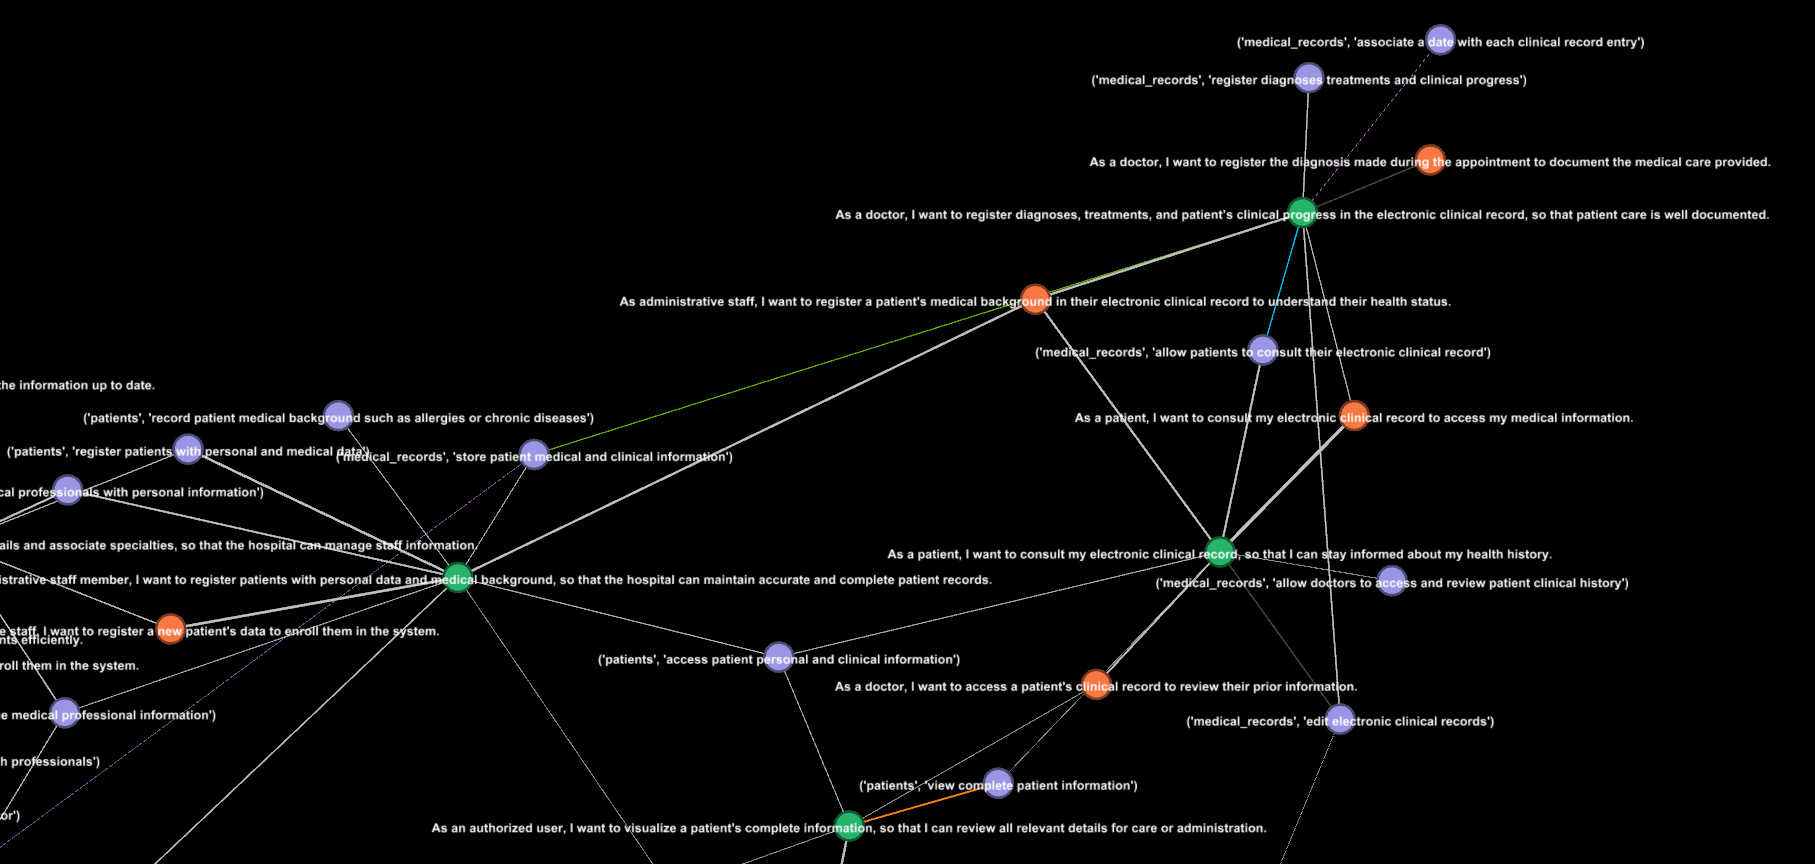
\includegraphics[width=\linewidth]{resultados/grafo/completo.png}
% \end{wrapfigure}

% Se construyó el gráfico para nuestra solución, con el fin de interpretar de manera gráfica los resultados obtenidos. El grafo completo está reportado en el Anexo (ref), pero ya que la visualización completa del mismo implica reducir mucho el tamaño de imagen, se analizan subgrafos representativos, que son partes del grafo completo resultado de la aplicación de la metodología.


% \subsubsection{Caso 1: Alineación semántica fuerte}
% \begin{wrapfigure}{r}{0.4\textwidth} % r = derecha, l = izquierda
%     \centering
%     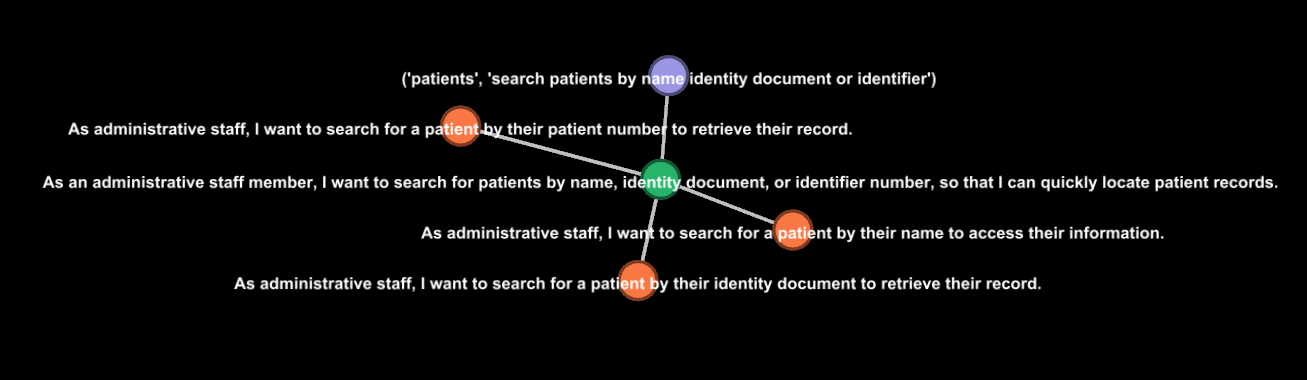
\includegraphics[width=0.38\textwidth]{resultados/grafo/pacientes.png}
%     \caption{Similitud semántica relativas a funcionalidades/historias correspondientes a Pacientes}
% \end{wrapfigure}

% Este

% \subsubsection{Caso 2: Cobertura parcial}
% \begin{wrapfigure}{r}{0.4\textwidth} % r = derecha, l = izquierda
%     \centering
%     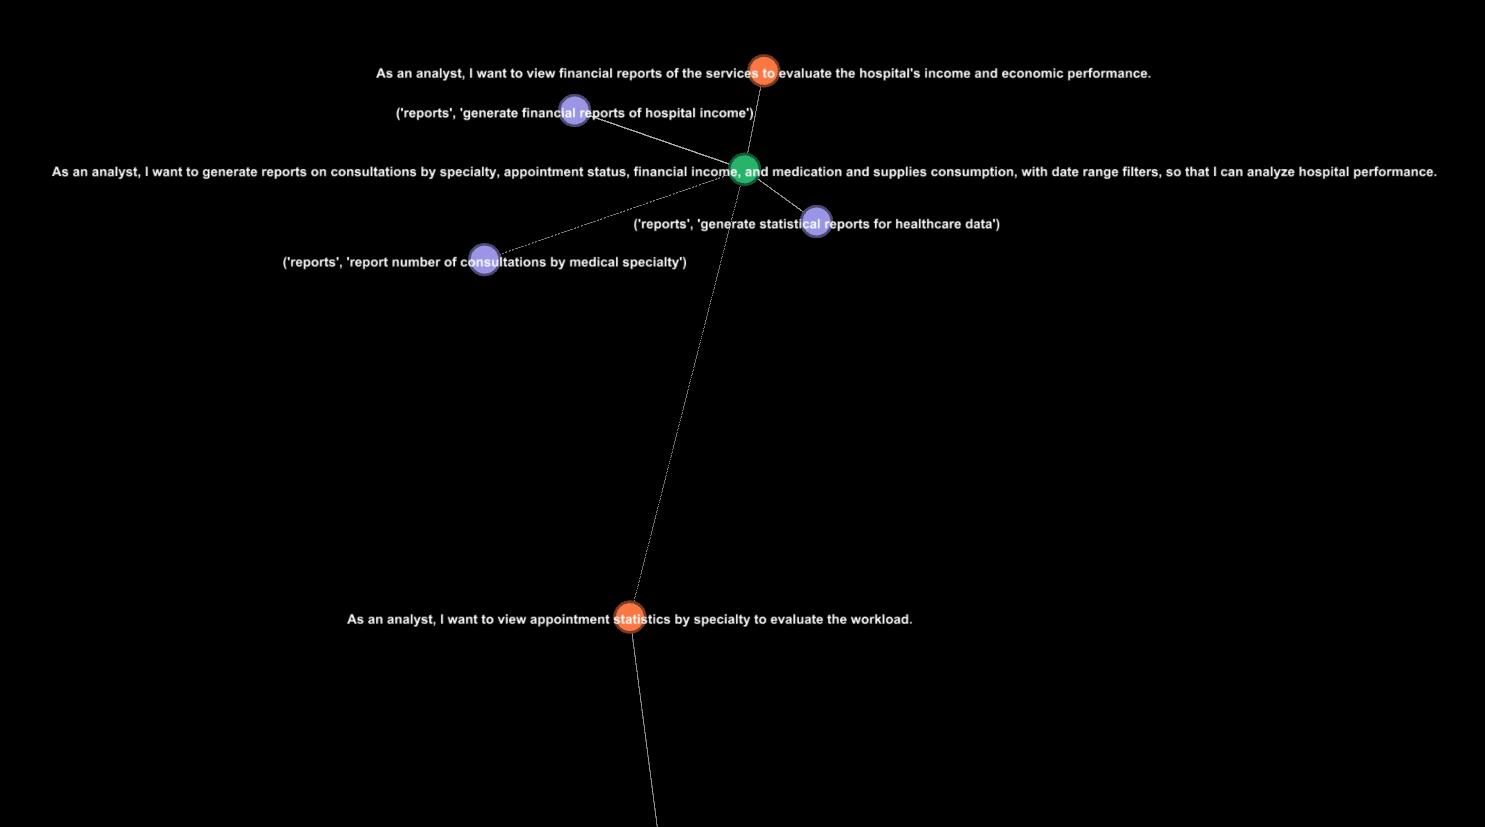
\includegraphics[width=0.38\textwidth]{resultados/grafo/coberturaParcial.png}
%     \caption{Ejemplo de cobertura parcial}
% \end{wrapfigure}

% Este

% \subsubsection{Caso 3: Funcionalidades no cubiertas}
% \begin{wrapfigure}{r}{0.4\textwidth} % r = derecha, l = izquierda
%     \centering
%     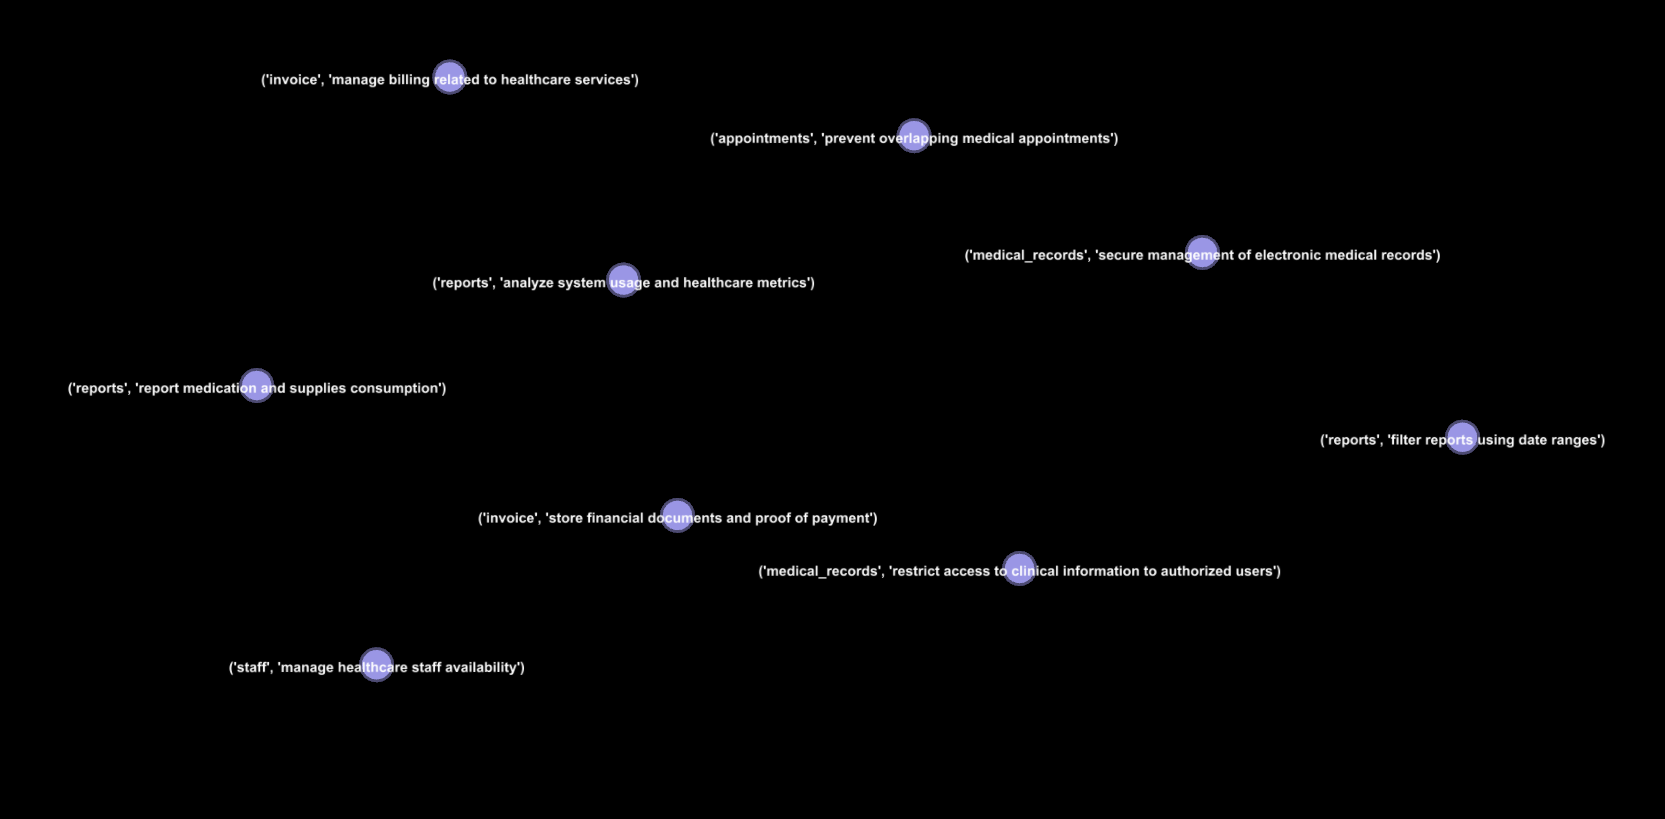
\includegraphics[width=0.38\textwidth]{resultados/grafo/funcionalidadesNoCubiertas.png}
%     \caption{Funcionalidades no cubiertas}
% \end{wrapfigure}

% Este

% \subsubsection{Caso 4: Potencial alucinación}
% \begin{wrapfigure}{r}{0.4\textwidth} % r = derecha, l = izquierda
%     \centering
%     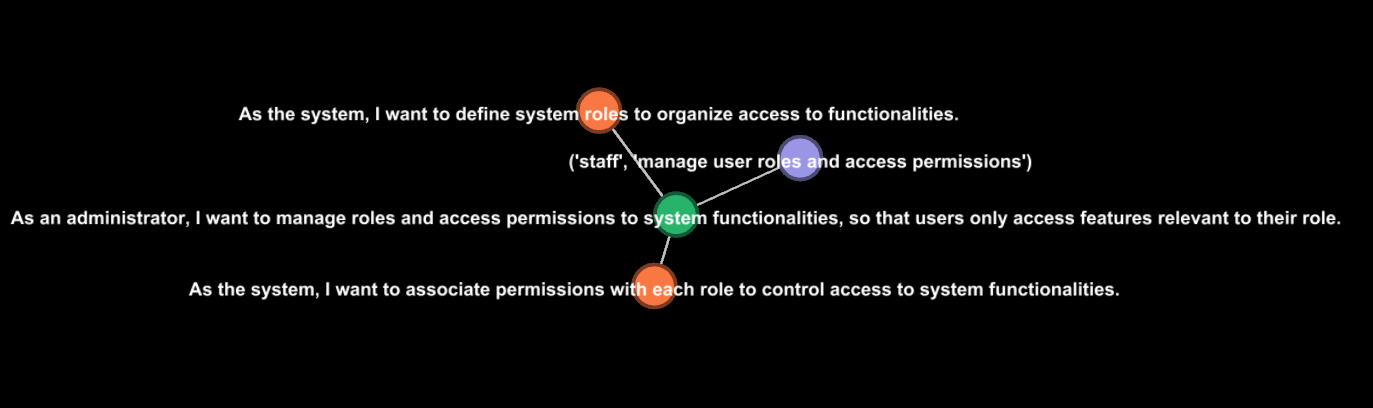
\includegraphics[width=0.38\textwidth]{resultados/grafo/roles.png}
%     \caption{Ejemplo de imagen}
% \end{wrapfigure}

% Este

\subsubsection{Discusión sobre Similitud Semántica}
Los resultados de la evaluación semántica son consistentes con las conclusiones de la evaluación manual en varios puntos concretos. La baja correspondencia en criterios de aceptación (10\% alineados) se corresponde con la baja estimabilidad encontrada en QUSF (42,9\%) e INVEST (9,5\%). La alta alineación de historias (92\% con al menos posible alineamiento) es coherente con lo observado en QUSF, donde la mayoría de las historias son conceptualmente sólidas y orientadas al problema, y en INVEST, donde el 95,2\% se considera negociable y valiosas. Por último, la detección de alucinaciones por similitud semántica identificó las mismas dos historias (HU22 y HU23) que el análisis manual. Esta consistencia entre ambos enfoques sugiere que la evaluación automática puede funcionar como un primer filtro antes de la revisión manual, ayudando a identificar los casos que necesitan más atención.

Por otro lado, los resultados también muestran limitaciones del uso de SBERT. Como se observó en los casos de alineación incorrecta, textos que comparten vocabulario pueden obtener valores de similitud altos a pesar de referirse a funcionalidades distintas, mientras que diferencias como quién realiza una acción o el nivel de detalle de una historia no son capturadas por el modelo. Esto debe tenerse en cuenta a la hora de interpretar los valores de similitud obtenidos.

\subsection{Análisis del grafo de similitud semántica}

El grafo de similitud semántica permite analizar la estructura de las relaciones entre historias generadas, historias esperadas y funcionalidades del dominio, esta representación aporta una visión complementaria al análisis basado en valores de similitud., lo que resulta útil para identificar patrones estructurales asociados a alineación, cobertura parcial y ausencia de correspondencias.

En general, el grafo presenta múltiples componentes conectados que corresponden a distintos subdominios funcionales (por ejemplo, pacientes, facturación, inventario y reportes). Dentro de estos componentes se observan agrupamientos densos, donde historias generadas, historias esperadas y funcionalidades se conectan mediante valores de similitud elevados, indicando una adecuada alineación semántica del modelo en estos casos.

\begin{figure}[H]
    \centering
    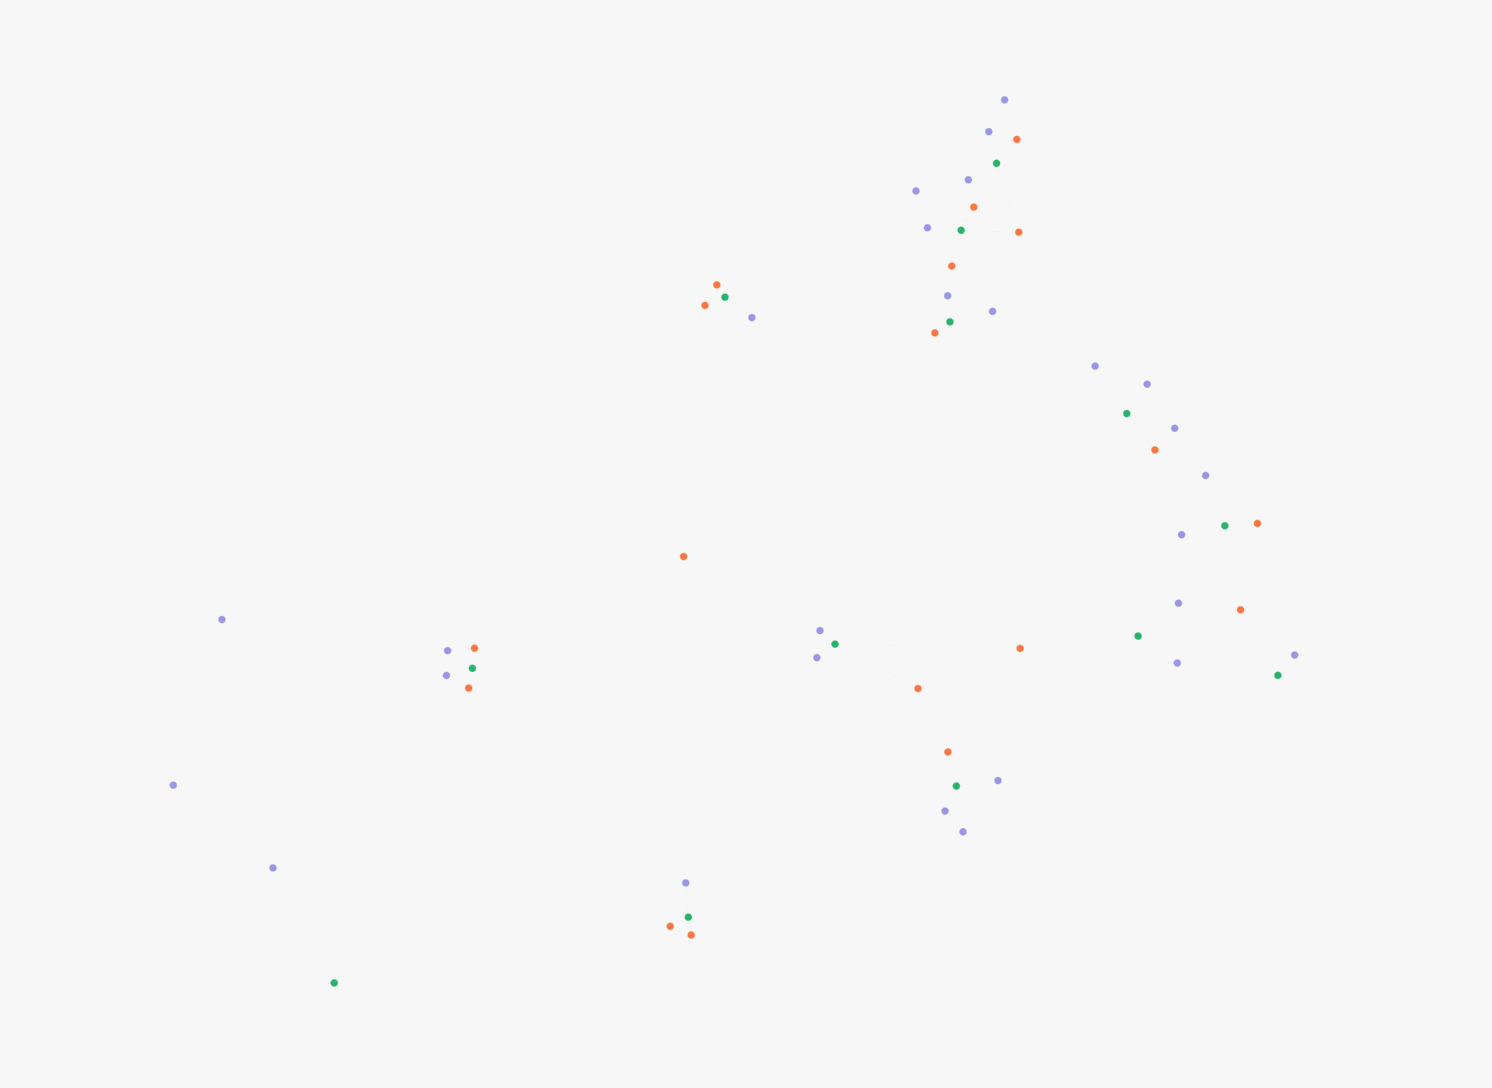
\includegraphics[width=\linewidth]{figs/grafo/vistaGeneral.png}
    \caption{Vista global del grafo de similitud semántica.}
    \label{fig:grafo_global}
\end{figure}

Sin embargo, el principal valor del grafo es la identificación de posibles inconsistencias respecto al  comportamiento esperado. Se observan nodos que no presentan conexiones significativas con el resto del grafo, es decir, nodos aislados. Estos nodos corresponden a elementos que no alcanzan los umbrales de similitud mínimos, lo que puede indicar una ausencia de correspondencia semántica para alguno de los elementos analizados.

\begin{figure}[H]
    \centering
    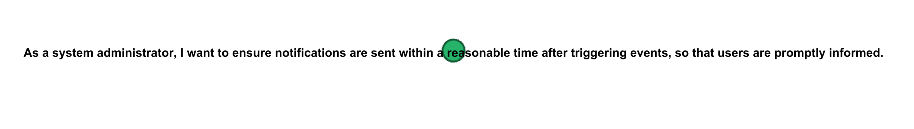
\includegraphics[width=0.7\linewidth]{figs/grafo/histGenAlucin1.png}
    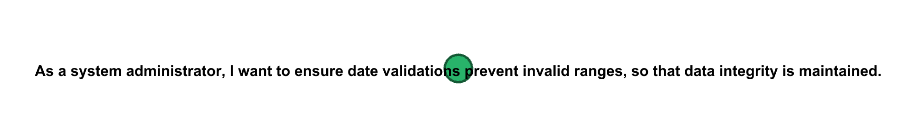
\includegraphics[width=0.7\linewidth]{figs/grafo/histGenAlucin2.png}
    \caption{Ejemplos de historias generadas sin correspondencia semántica.}
    \label{fig:alucinaciones}
\end{figure}

El análisis de estos casos permite validar la consistencia del grafo con los resultados previamente discutidos en la sección de detección de alucinaciones. Particularmente, las historias:

\begin{itemize}
    \item ``As a system administrator, I want to ensure notifications are sent within a reasonable time after triggering events...''
    \item ``As a system administrator, I want to ensure date validations prevent invalid ranges...''
\end{itemize}

aparecen como nodos aislados en el grafo, sin conexiones hacia funcionalidades ni historias esperadas. Este comportamiento indica que dichas historias no presentan similitud semántica suficiente con el dominio funcional definido. Esto se corresponde con el análisis de alucinaciones realizado, donde se identificaron estas historias como contenido no alineado con los requerimientos del sistema. En resumen, el grafo confirma que se trata de posibles alucinaciones del modelo, es decir historias generadas que no pueden ser correspondidas a ninguna historia esperada ni funcionalidad definida. :contentReference[oaicite:0]{index=0}

\begin{figure}[H]
    \centering
    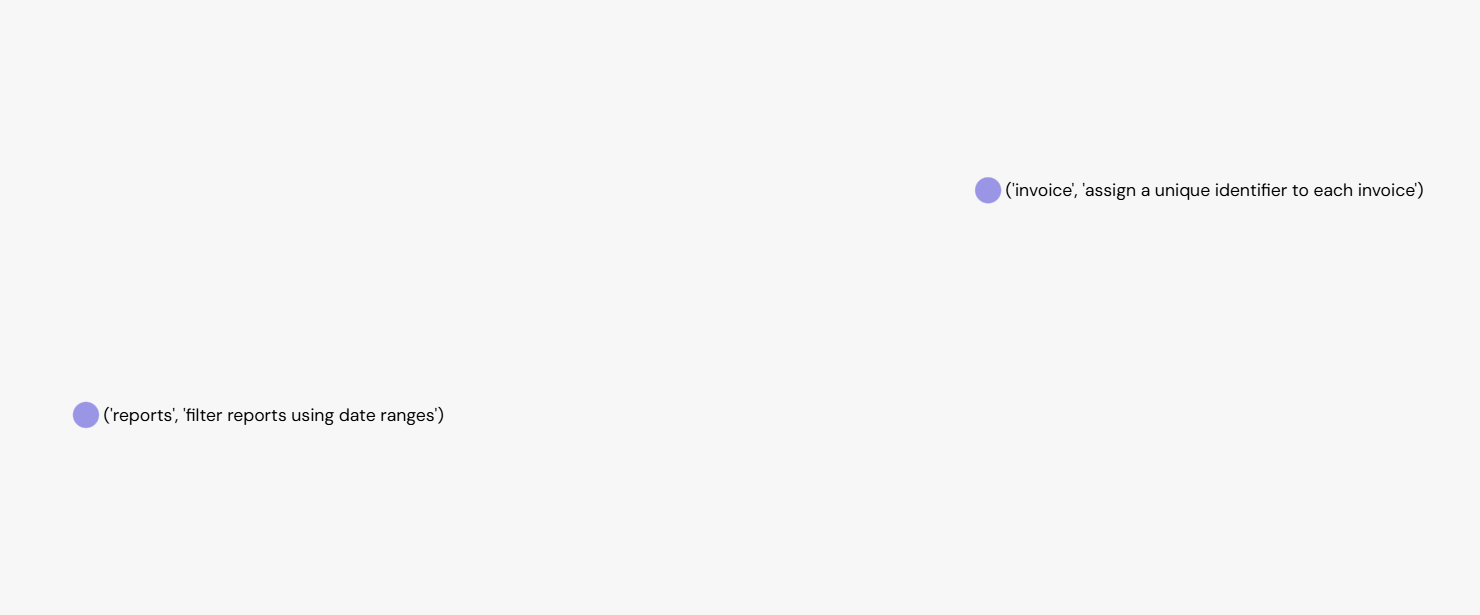
\includegraphics[width=0.7\linewidth]{figs/grafo/alucionaciones1.png}
    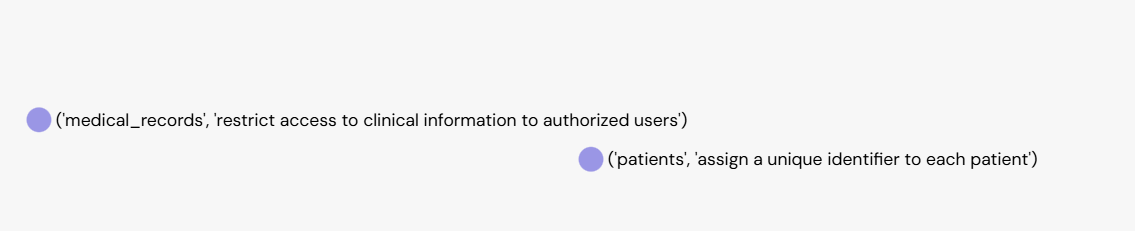
\includegraphics[width=0.7\linewidth]{figs/grafo/alucinaciones2.png}
    \caption{Ejemplos de historias generadas sin correspondencia semántica.}
    \label{fig:alucinaciones}
\end{figure}

En la anterior figura se pueden también identificar casos en los que funcionalidades o historias esperadas no presentan conexiones con historias generadas. En estos casos, el grafo evidencia una falta de cobertura del modelo, indicando que ciertos requerimientos del dominio no han sido representados correctamente en la salida generada. 

Además se observan situaciones donde las conexiones existen pero presentan valores de similitud intermedios y se distribuyen entre múltiples nodos, en estos casos no se identifica una correspondencia clara, sino una dispersión de relaciones semánticas.


\begin{figure}[H]
    \centering
    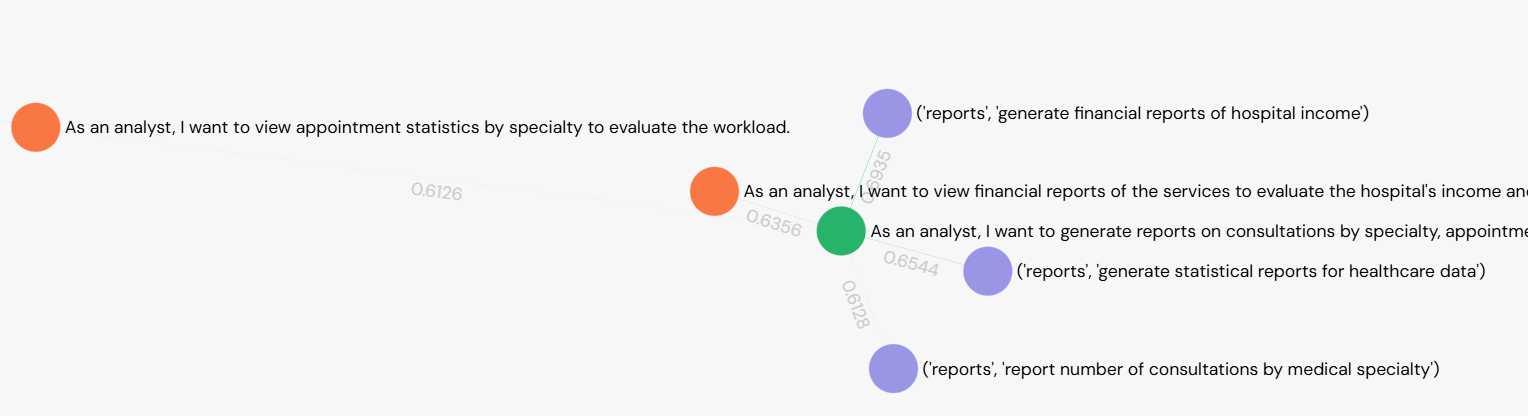
\includegraphics[width=0.9\linewidth]{figs/grafo/reportes.png}
    \caption{Ejemplo de cobertura parcial con similitudes distribuidas.}
    \label{fig:ambiguedad}
\end{figure}

Finalmente, también se identifican casos donde una única historia generada se conecta con múltiples funcionalidades o historias esperadas. Este comportamiento indica una agregación de requerimientos en una sola historia, lo que sugiere que la generación de historias por parte del modelo tiende a agrupar mas de una funcionalidad si las mismas están relacionadas.

\begin{figure}[H]
    \centering
    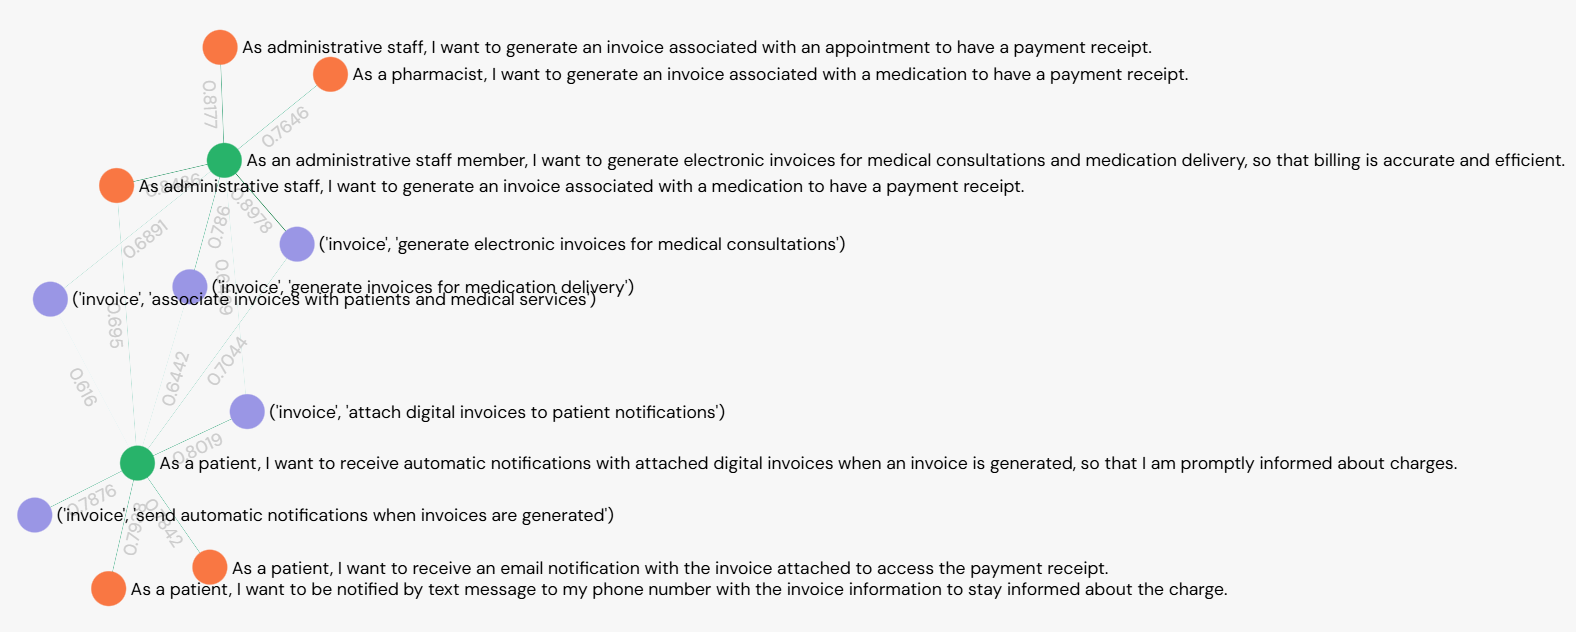
\includegraphics[width=0.9\linewidth]{figs/grafo//facturas.png}
    \caption{Ejemplo de historia generada con múltiples correspondencias.}
    \label{fig:epica}
\end{figure}

En conjunto, el grafo permite identificar tres comportamientos relevantes del modelo: (i) alineación correcta, evidenciada por agrupamientos densos, (ii) cobertura parcial, que se puede identificar por conexiones distribuidas con similitud intermedia, y (iii) ausencia de correspondencia, lo que se logra identificar mediante nodos aislados, estos casos de nodos aislados son además consistentes con el análisis previo, en el que las dos historias catalogadas como alucinación son las mismas que el grafo representó como nodos aislados.